\chapter{Informatik -- Worum geht's?}
\renewcommand{\chaptertitle}{Informatik -- Worum geht's}

\lehead[]{\normalfont\sffamily\hspace*{-2.00cm}\textcolor{white}{\colorbox{lightblue}{\makebox[1.60cm][r]{\thechapter}}}\hspace{0.17cm}\textcolor{lightblue}{\chaptertitle}}
\rohead[]{\textcolor{lightblue}{\chaptertitle}\normalfont\sffamily\hspace*{0.17cm}\textcolor{white}{\colorbox{lightblue}{\makebox[1.60cm][l]{\thechapter}}}\hspace{-2.00cm}}
%\chead[]{}
\rehead[]{\textcolor{lightblue}{AvHG, Inf, My}}
\lohead[]{\textcolor{lightblue}{AvHG, Inf, My}}


\section{Informatik}

\subsection{Gegenstand der Informatik}

Die meisten Menschen denken bei Informatik sofort an Computer. Das ist nicht ganz
falsch, denn Computer sind als Werkzeug für die Informatik von zentraler Bedeutung.

Dem gegenüber steht jedoch ein bekanntes Zitat des niederländischen Informatikers
Edsger Wybe Dijkstra:

\begin{quotation}
\noindent In der Informatik geht es genauso wenig um Computer wie in der
Astronomie um Teleskope.
\end{quotation}

Dieses Zitat verdeutlicht den reinen Werkzeugcharakter des Computers.

Die Informatik beschäftigt sich als Wissenschaft mit der \textbf{systematischen und
automatisierten Verarbeitung von Informationen}. Um Informationen automatisiert
verarbeiten zu können, braucht es zwei Dinge: zum einen geeignete Maschinen
(Computer) und zum anderen genaue, eindeutige Handlungsanweisungen, wie die Daten
verarbeitet werden sollen.

Eine solche eindeutige Handlungsanweisung zur Lösung eines Problems nennt man
\emph{Algorithmus}. Dies ist einer der wichtigsten Grundbegriffe der Informatik.


\subsection{Teilgebiete der Informatik}

\begin{figure}[h]
  \centering
   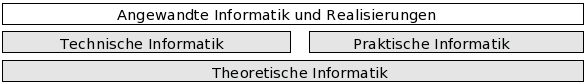
\includegraphics[width=1.0\textwidth]{./inf/SEKII/03_Informatik/Architektur-der-Informatik.png}
   \caption{Teilgebiete der Informatik}
   %
   % http://de.wikipedia.org/wiki/Informatik#mediaviewer/Datei:Architektur-der-informatik.png, Erstellt von Matthias Kleine. Lizenziert unter Creative Commons Attribution-Share Alike 3.0
\end{figure}
% http://de.wikipedia.org/wiki/Informatik#mediaviewer/Datei:Architektur-der-informatik.png

Im Informatikunterricht beschäftigen wir uns schwerpunktmäßig mit Themen der
\emph{Praktischen Informatik}. Mit anderen Worten: Ihr werdet lernen, passende
Algorithmen für gegebene Probleme zu entwickeln und diese in einer
Programmiersprache umzusetzen (zu implementieren).

Darüber hinaus werfen wir auch Blicke in die anderen Teilgebiete der Informatik:

\begin{compactitem}
\item[\emph{Theoretische Informatik}:]\hspace{1cm}
  \begin{compactitem}
  \item Aussagenlogik
  \item Kryptologie (Verschlüsselung)
  \end{compactitem}
\item[\emph{Technische Informatik}:]\hspace{1cm}
  \begin{compactitem}
  \item Rechnerarchitektur (Aufbau eines Computers)
  \item Aufgaben und Funktionsweise von Betriebssystemen
  \item Netzwerkprotokolle (wie das Internet funktioniert)
  \end{compactitem}
\item[\emph{Angewandte Informatik}:]\hspace{1cm}
  \begin{compactitem}
  \item Datenschutz und Urheberrecht
  \item Informatik und Gesellschaft (z.\,B.\ Künstliche Intelligenz)
  \item Anwendungsgebiete in Wirtschaft und Wissenschaft
  \end{compactitem}
\end{compactitem}


\section{Was Computer eigentlich können}

Streng genommen können Computer nur zwei Dinge tun:

\begin{compactenum}[1.]
\item Sehr einfache Berechnungen ausführen.
\item Sich die Ergebnisse solcher Berechnungen merken.
\end{compactenum}

Das klingt zunächst nach wenig. Diese beiden Dinge können Computer allerdings
\emph{extrem} gut! Ein moderner PC führt pro Sekunde rund 50 Milliarden
Rechenoperationen aus. Selbst in der unvorstellbar kurzen Zeit, die das Licht
braucht, um von der Schreibtischlampe auf eine nur 60 Zentimeter entfernte
Tischplatte zu treffen, hat ein aktueller PC bereits rund 100 Berechnungen
durchgeführt. Und dabei ist Licht unfassbar schnell: Pro Sekunde legt es eine
Entfernung von 300.000 Kilometern zurück -- damit könnte man die Erde in einer
einzigen Sekunde fast achtmal umrunden!

Über Jahrtausende hinweg waren die Möglichkeiten, Berechnungen anzustellen,
durch die Geschwindigkeit des menschlichen Gehirns begrenzt. Komplexere Probleme
waren schlicht nicht bewältigbar. Zwar gibt es auch heute noch Aufgaben, die für
Computer extrem schwierig oder kaum exakt lösbar sind -- wie etwa präzise
langfristige Wetter- und Klimavorhersagen aufgrund der riesigen Datenmengen und
chaotischen Wechselwirkungen. Dennoch erschließt die stetig wachsende
Rechenleistung immer neue Anwendungsfelder.

Im Inneren kennt ein Computer dabei nur zwei Zustände: Strom fließt oder Strom
fließt nicht (dargestellt als \textbf{1} und \textbf{0}). Doch genau damit lassen
sich Zahlen darstellen -- und wenn man Buchstaben, Töne, Bilder oder Messwerte
geschickt in Zahlen übersetzt (codiert), kann ein Computer nahezu jede Form von
\emph{Information} verarbeiten.


\section{Computational Thinking}

\emph{Computational Thinking} (oft als „informatisches Denken“ übersetzt)
beschreibt die Fähigkeit, auch alltägliche oder fachfremde Problemstellungen so zu
strukturieren, dass sie systematisch -- und im Idealfall mithilfe eines Computers --
gelöst werden können.

Populär wurde der Begriff durch die Informatikerin Jeannette Wing (damals Leiterin
des Computer Science Departments an der Carnegie Mellon University in Pittsburgh,
USA). In einem Interview mit der österreichischen Tageszeitung \emph{Der Standard}
vom 28.\ September 2010 erklärte sie die Bedeutung dieser Denkweise:

\begin{quotation}
\noindent Wer analytisch und präzise wie ein Computerwissenschafter denken
lernt, kann komplexe Probleme effizienter lösen.

\noindent Mit dem Denkmodell könnten selbst alltägliche Aufgaben wie das
Kaffeeholen in der Cafeteria effizienter gestaltet werden. Den Unterschied zu
gewissermaßen \glqq herkömmlichem\grqq\ logischem Denken erklärt Wing mit dem
herausragenden Stellenwert von Effizienz in der Computerwissenschaft:
\glqq Computational Thinking befähigt dazu, Strukturen und Muster zu erkennen,
wo man vorher keine gesehen hat, oder effizienter in der täglichen Routine zu
sein.\grqq

\noindent Besonderes Augenmerk legt die Wissenschaftlerin auf die
Implementierung ihres Konzeptes in das Bildungswesen. \glqq Zusätzlich zu den
Fertigkeiten wie Schreiben, Rechnen und Lesen sollte in Zukunft jedes Kind als
weitere analytische Fähigkeit die grundlegenden Konzepte der
Computerwissenschaften verinnerlichen\grqq .

\noindent \glqq Wenn wir lernen, schriftlich zu dividieren oder zwei große
Zahlen zu multiplizieren, lernen wir eigentlich einen Algorithmus. Nur sagt uns
das niemand\grqq , so Wing.
\end{quotation}

\noindent Quelle: \url{http://derstandard.at/1285199497847/}

\medskip
\noindent Konkret besteht \emph{Computational Thinking} aus vier Schritten, die
euch im Unterricht immer wieder begegnen werden:
\begin{compactenum}[1.]
\item \textbf{Zerlegung (Dekomposition):} Ein großes, unübersichtliches Problem in
kleine, handhabbare Teilprobleme aufteilen.
\item \textbf{Mustererkennung:} Ähnlichkeiten und wiederkehrende Abläufe innerhalb
dieser Teilprobleme entdecken.
\item \textbf{Abstraktion:} Unwichtige Details weglassen und sich auf das
Wesentliche konzentrieren.
\item \textbf{Algorithmenentwurf:} Eine klare Schritt-für-Schritt-Anleitung zur
Lösung formulieren.
\end{compactenum}
